% XCircuit output "BJT_struktura_1D.tex" for LaTeX input from BJT_struktura_1D.ps
\def\putbox#1#2#3#4{\makebox[0in][l]{\makebox[#1][l]{}\raisebox{\baselineskip}[0in][0in]{\raisebox{#2}[0in][0in]{\scalebox{#3}{#4}}}}}
\def\rightbox#1{\makebox[0in][r]{#1}}
\def\centbox#1{\makebox[0in]{#1}}
\def\topbox#1{\raisebox{-0.60\baselineskip}[0in][0in]{#1}}
\def\midbox#1{\raisebox{-0.20\baselineskip}[0in][0in]{#1}}
   \scalebox{0.8}{
   \normalsize
   \parbox{3.47917in}{
   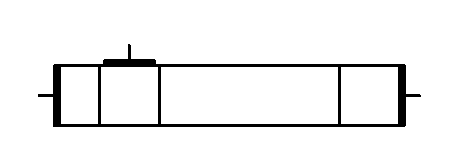
\includegraphics[scale=1.25]{BJT_struktura_1D}\\
   % translate x=359 y=239 scale 0.30
   \putbox{0.06in}{0.27in}{1.20}{E}%
   \putbox{0.88in}{0.77in}{1.20}{B}%
   \putbox{3.40in}{0.27in}{1.20}{C}%
   \putbox{0.40in}{0.23in}{1.20}{N$^+$}%
   \putbox{0.86in}{0.23in}{1.20}{P}%
   \putbox{1.52in}{0.23in}{1.20}{N$^-$- drift}%
   \putbox{2.81in}{0.23in}{1.20}{N$^+$}%
   } % close 'parbox'
   } % close 'scalebox'
   \vspace{-\baselineskip} % this is not necessary, but looks better
